\chapter{Resultados y análisis}

\section{Evidencia disponible para OLS y Ridge}

Se analizaron las gráficas almacenadas junto a los programas descritos en la sección~\ref{sec:metodo-lineales}. Estas imágenes constituyen salidas conservadas de ejecuciones previas; no se dispone en ellas de una identificación de la versión del programa, del conjunto exacto de datos ni de las métricas numéricas. Por ello, la asociación se establece por los nombres de archivo y se limita a una interpretación visual.

\subsection{Salidas de un paso}

\begin{figure}[htbp]
\centering
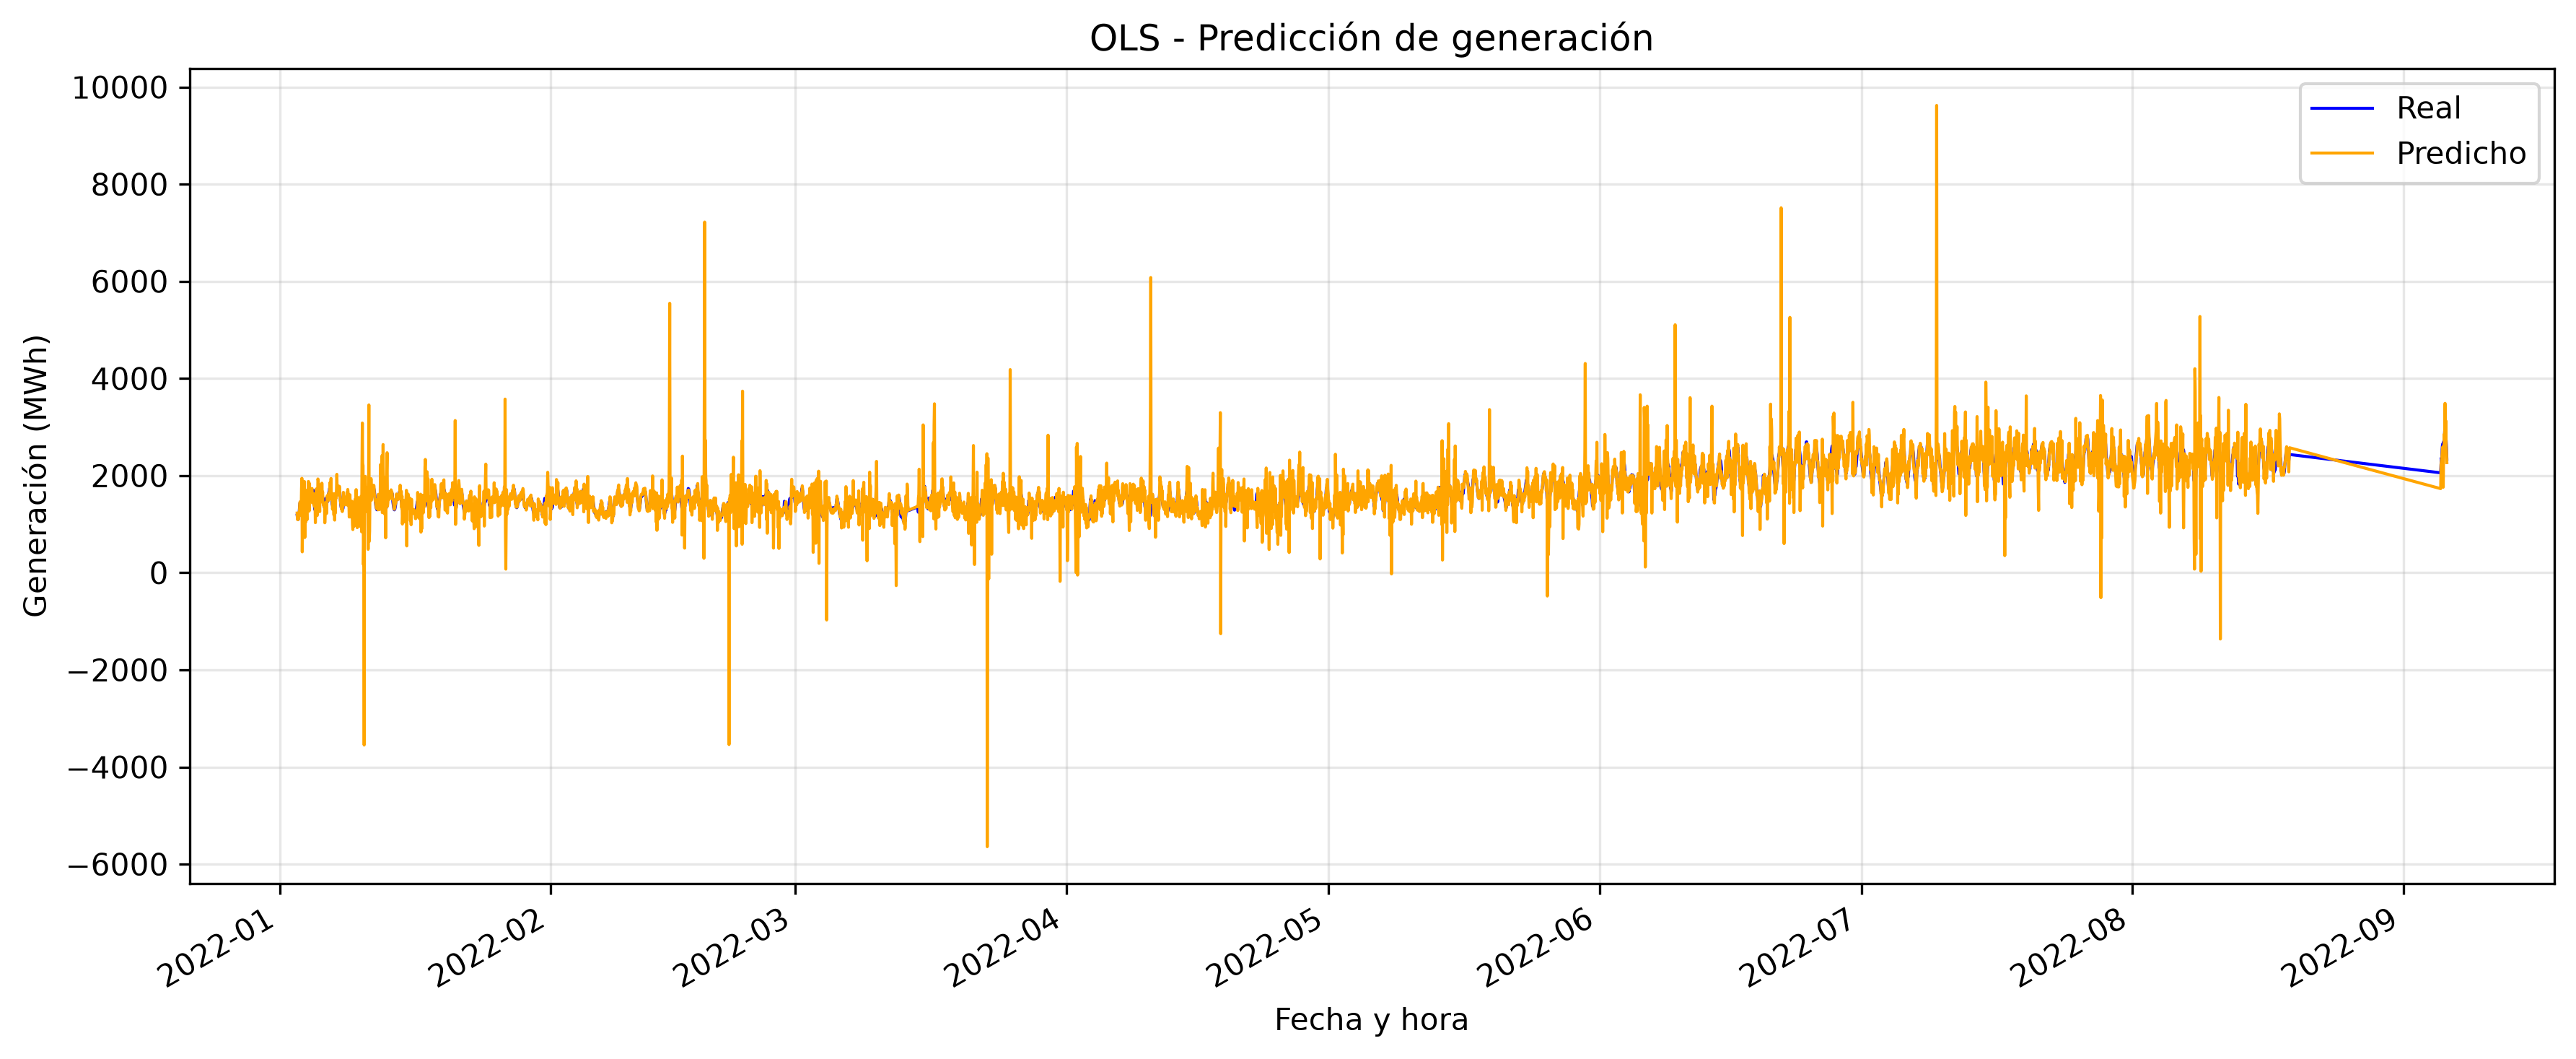
\includegraphics[width=\textwidth]{codigos de docker/root/prediccion_vs_real_ols.png}
\caption{Salida conservada de OLS para la comparación entre generación observada y estimada. El eje horizontal representa la secuencia de predicciones.}
\label{fig:ols-un-paso}
\end{figure}

En la figura~\ref{fig:ols-un-paso}, la trayectoria estimada reproduce visualmente las oscilaciones generales y el aumento de nivel hacia la parte final de la secuencia. Se observan diferencias locales en máximos y mínimos. La superposición de trazos permite examinar el seguimiento global, pero no establece por sí sola la magnitud del error ni la ausencia de sesgo.

\begin{figure}[htbp]
\centering
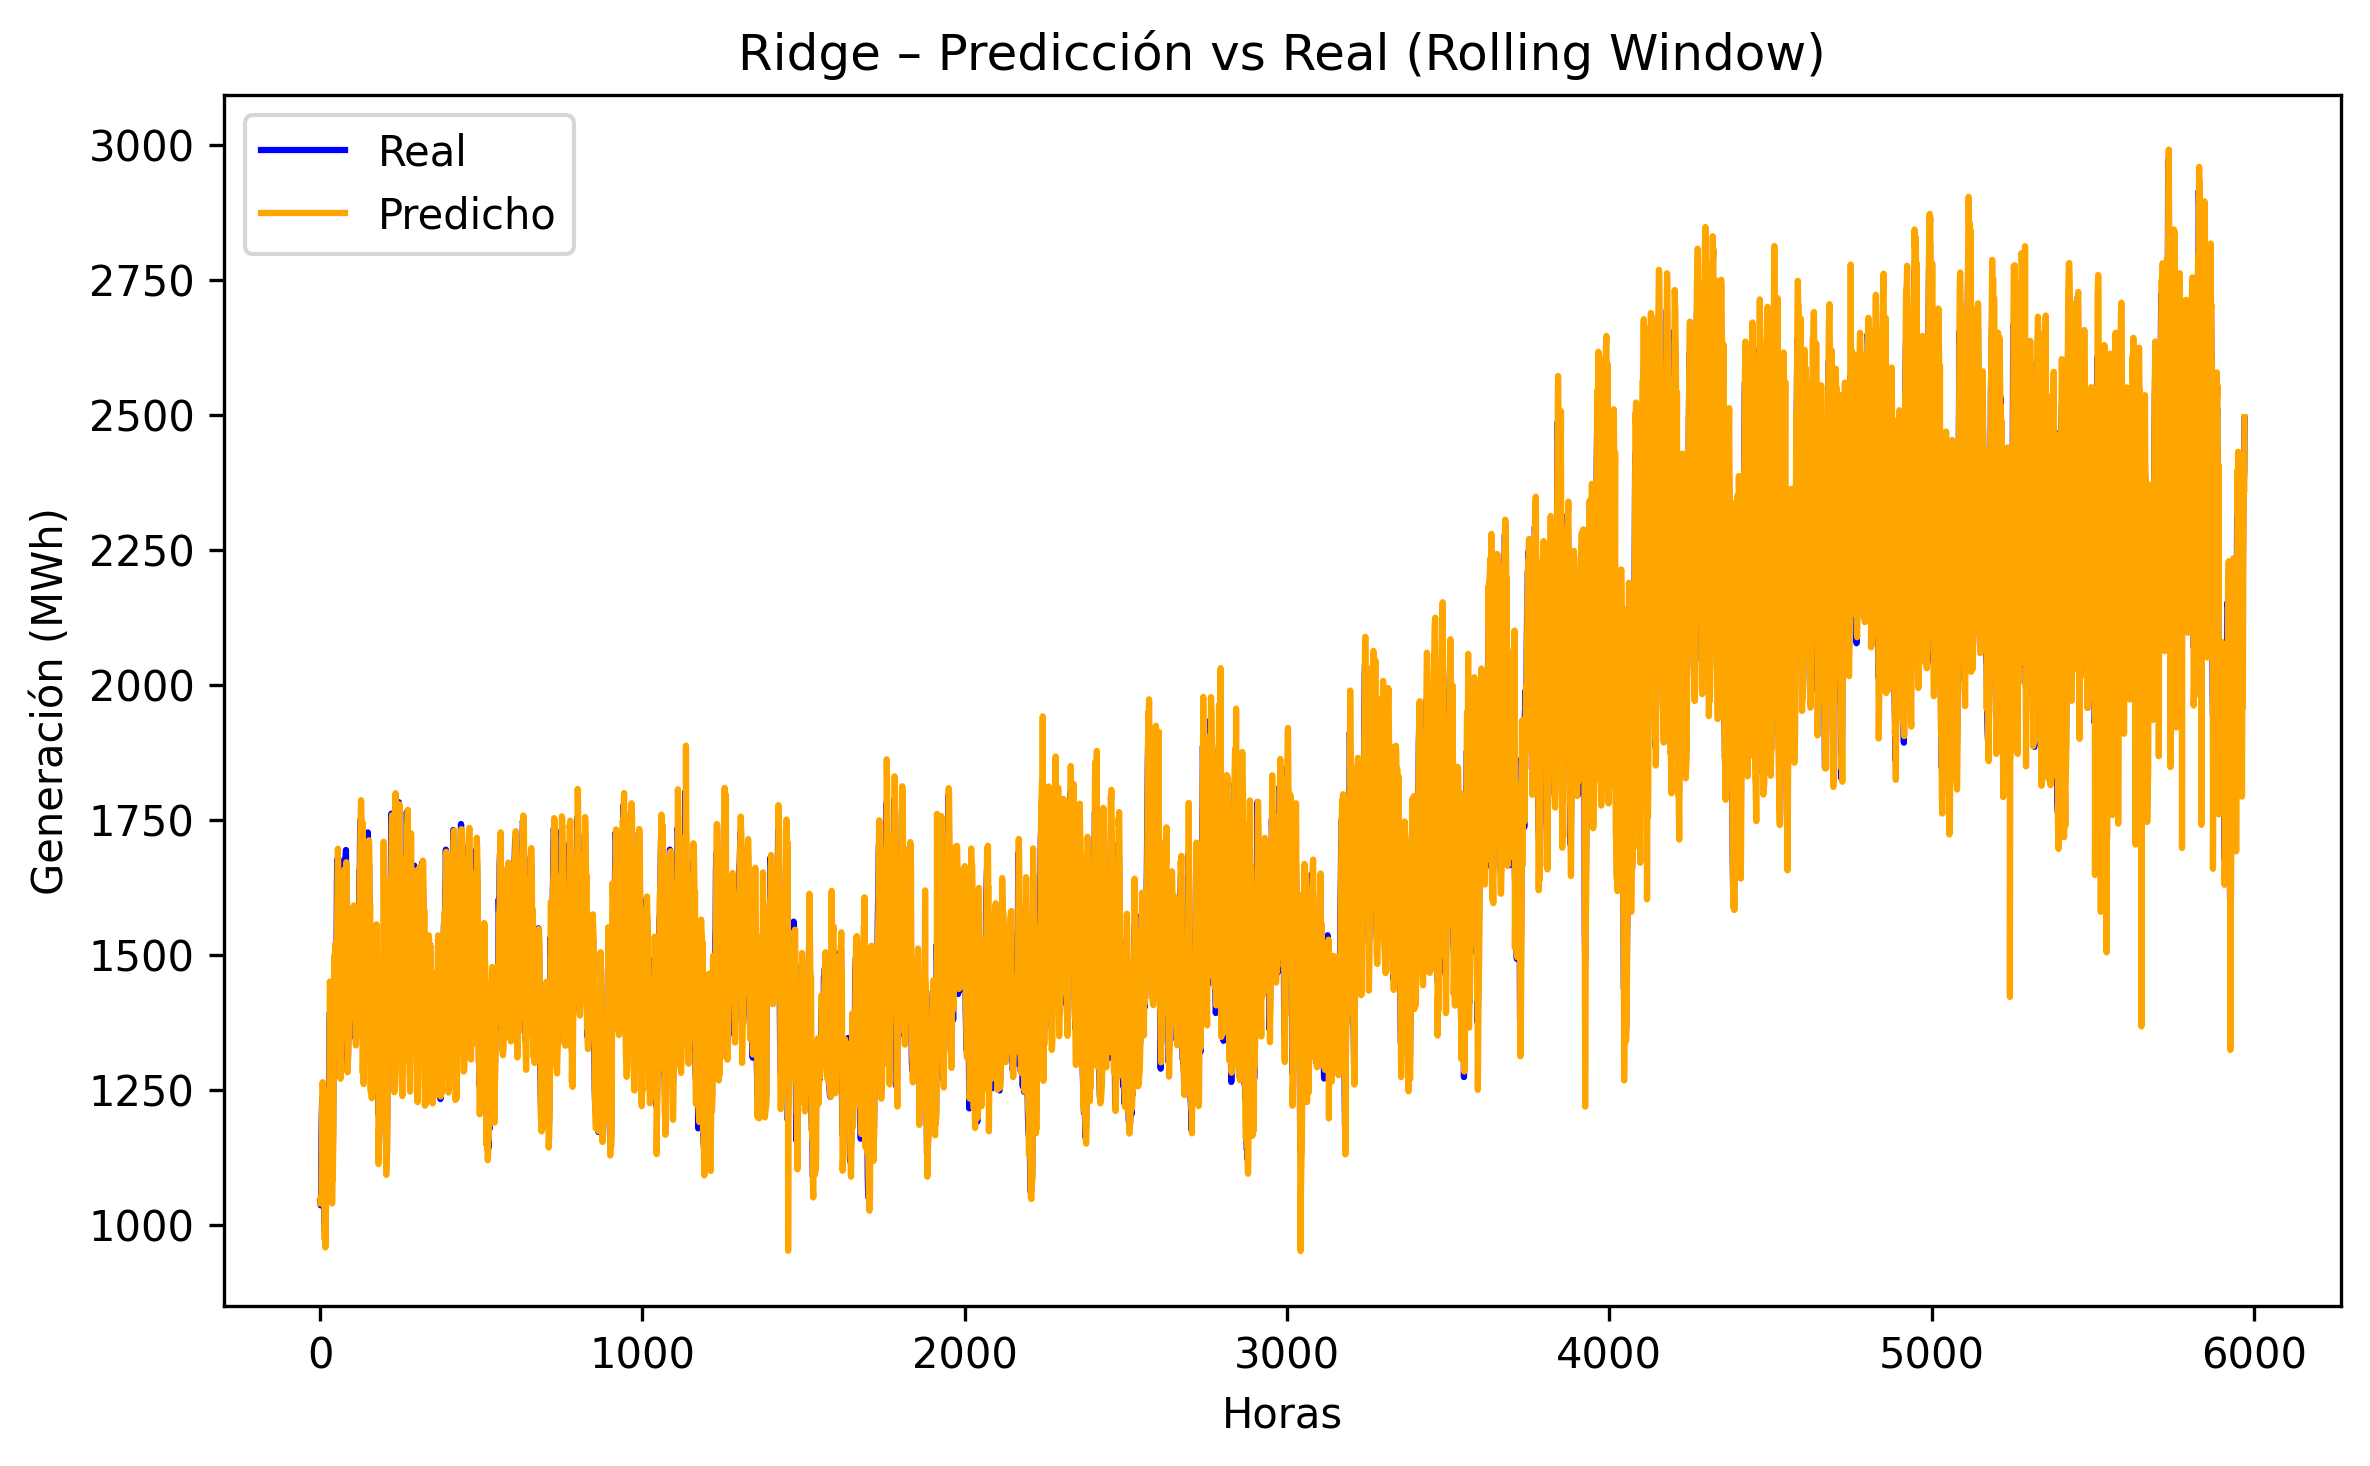
\includegraphics[width=\textwidth]{codigos de docker/root/prediccion_vs_real_ridge.png}
\caption{Salida conservada de Ridge con ventana móvil. La alta superposición de curvas limita la identificación visual de errores puntuales.}
\label{fig:ridge-un-paso}
\end{figure}

La figura~\ref{fig:ridge-un-paso} presenta una superposición amplia entre valores observados y estimados, tanto en el tramo de menor generación como en el de mayor nivel. Este comportamiento es compatible con un seguimiento cercano de la serie representada, aunque no permite concluir que Ridge supera a OLS. Además de no contar con métricas verificables para estas imágenes, los programas difieren en entradas, longitud de historia y escalamiento.

\subsection{Salidas de diez pasos}

\begin{figure}[htbp]
\centering
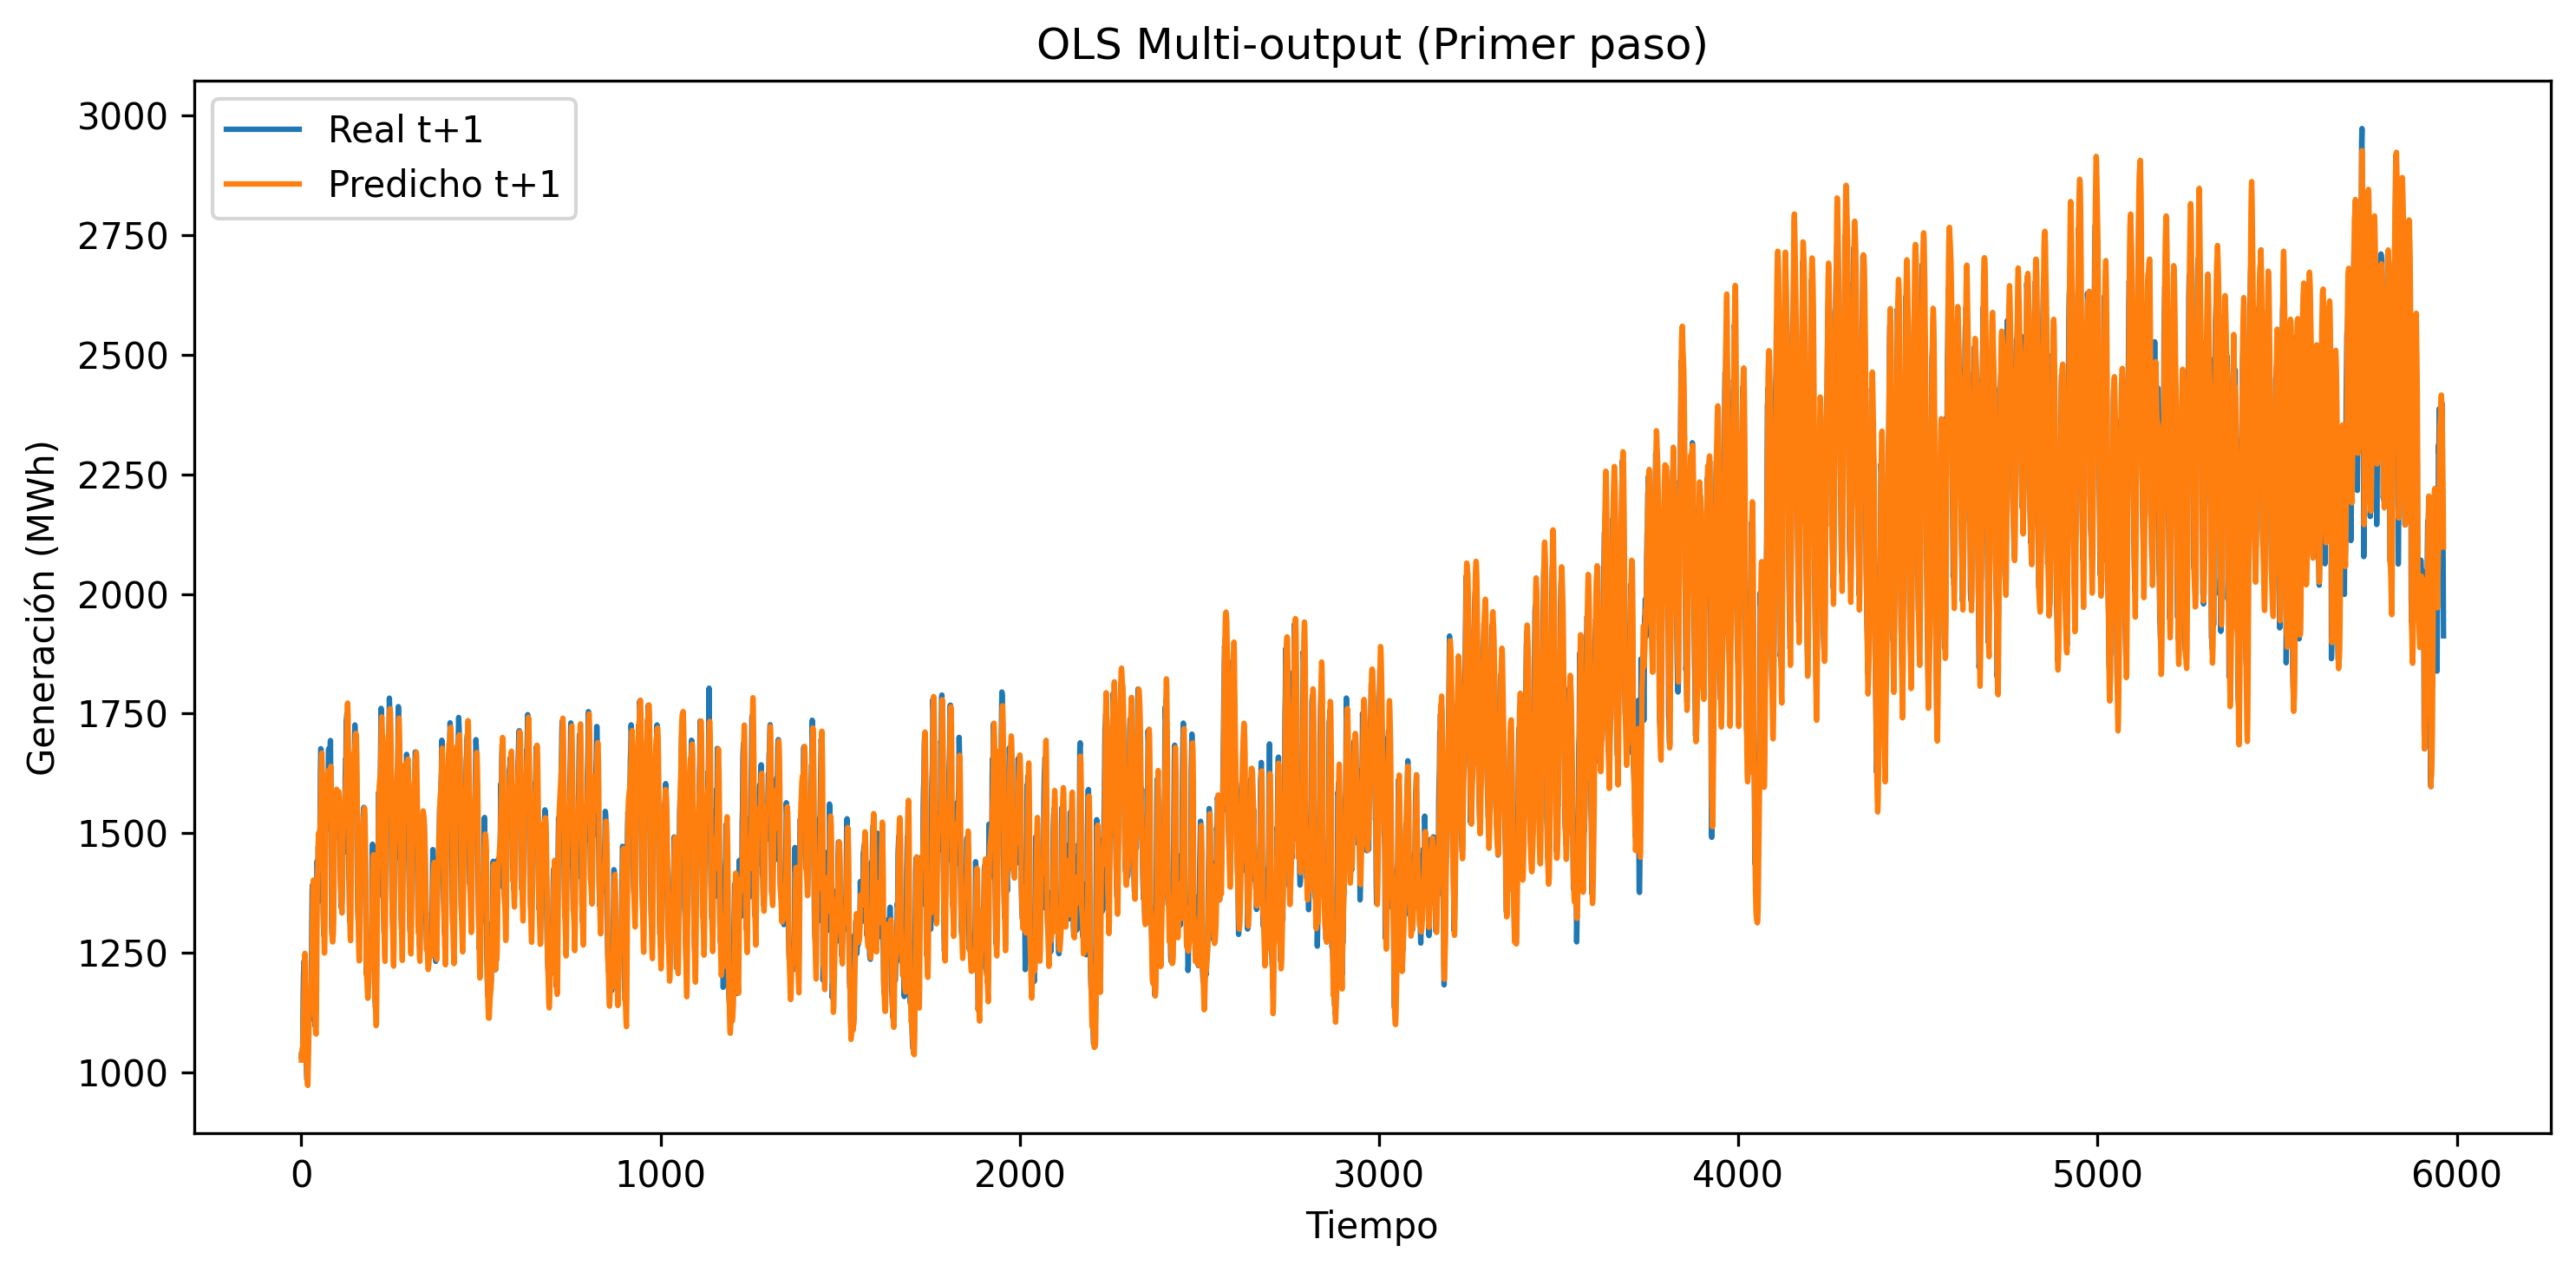
\includegraphics[width=\textwidth]{codigos de docker/root/prediccion_ols_multioutput.png}
\caption{Primer componente de la salida múltiple de OLS. La construcción de las respuestas incluye datos del intervalo evaluado.}
\label{fig:ols-multi}
\end{figure}

\begin{figure}[htbp]
\centering
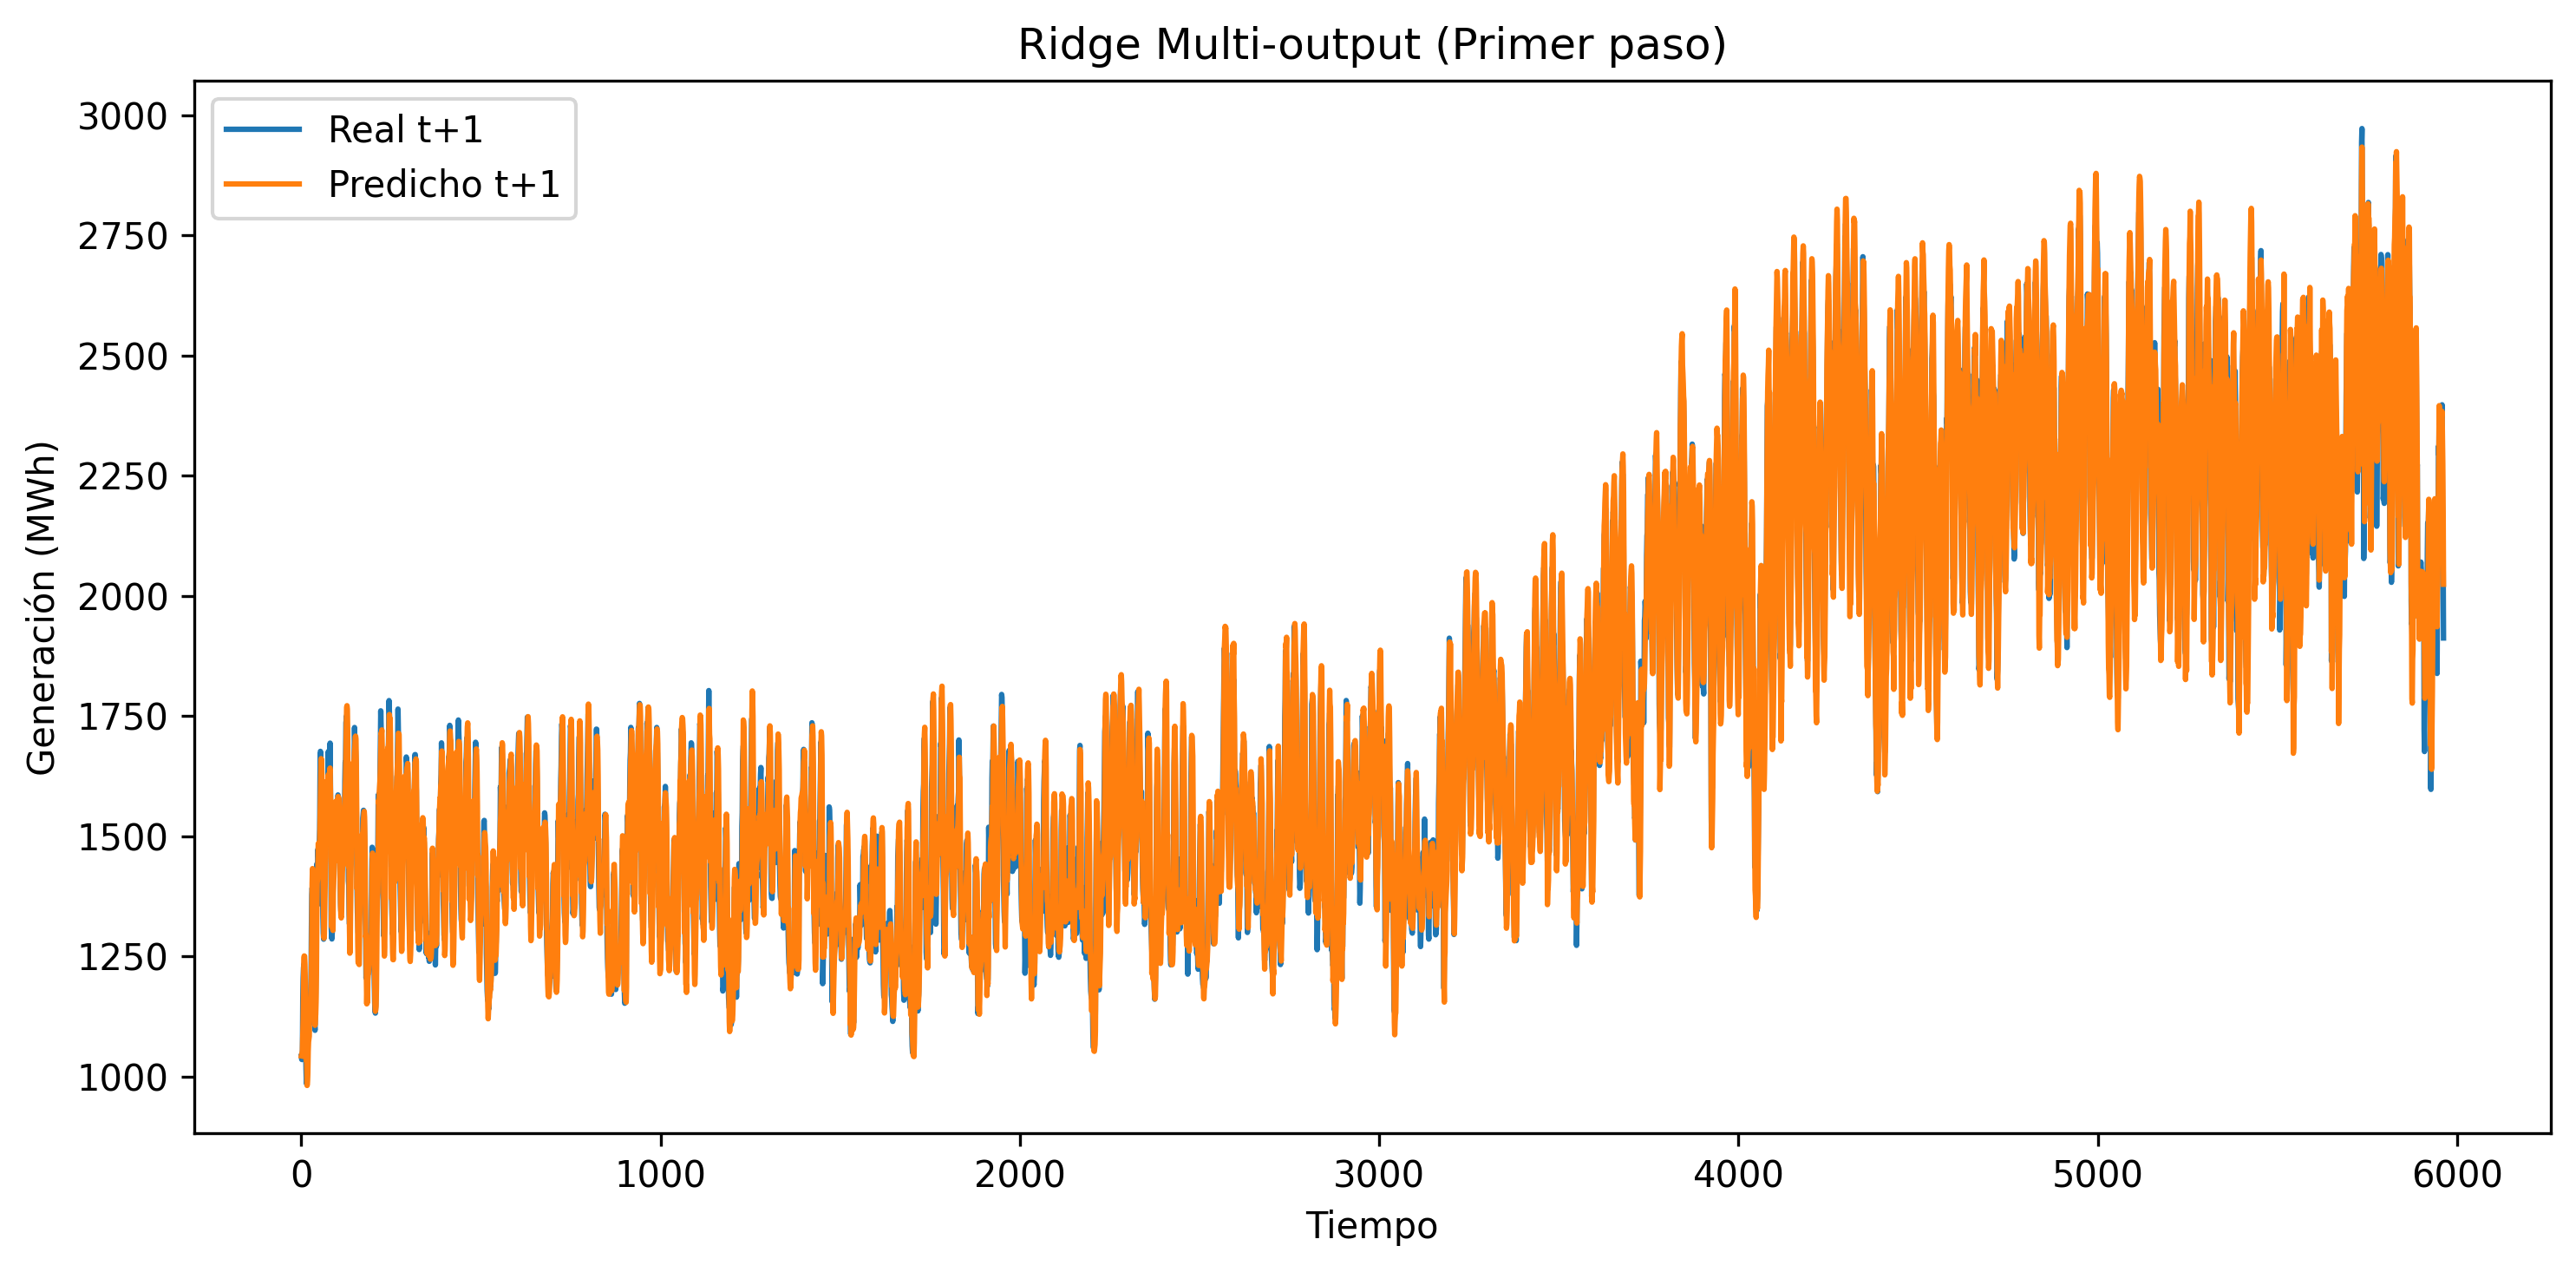
\includegraphics[width=\textwidth]{codigos de docker/root/prediccion_ridge_multioutput.png}
\caption{Primer componente de la salida múltiple de Ridge. Esta gráfica no representa el desempeño de los diez horizontes por separado.}
\label{fig:ridge-multi}
\end{figure}

Las figuras~\ref{fig:ols-multi} y~\ref{fig:ridge-multi} muestran cercanía entre las curvas del primer componente. Sin embargo, la fuga de información identificada en la subsección~\ref{subsec:lineales-multi} condiciona su interpretación: la coincidencia no demuestra capacidad de generalización a datos futuros. Tampoco permite inferir el comportamiento de los pasos segundo a décimo, ausentes en las imágenes.

\section{Alcance de la comparación}

Los archivos breves \texttt{resultados.txt} de la carpeta principal de códigos y de \texttt{ya emp} contienen métricas de transformadores, que no se atribuyeron a OLS ni a Ridge. No se transcribieron cifras estimadas a partir de las gráficas. Queda pendiente incorporar las salidas numéricas de consola de los experimentos lineales con una identificación inequívoca de programa, datos y ejecución.

La evidencia revisada permite describir la implementación y su comportamiento visual, pero no establecer una clasificación cuantitativa entre los dos modelos. Para interpretar resultados posteriores deberán distinguirse los experimentos de ventana móvil con reajuste, los de ajuste único con rezagos y los de salida múltiple. En particular, las salidas exploratorias con información compartida entre ajuste y evaluación deben mantenerse separadas de las pruebas independientes.

\section{Otros modelos}

El análisis de las arquitecturas restantes se incorporará después de documentar sus procedimientos y las salidas disponibles.
